% !TEX encoding = UTF-8 Unicode
% !TEX spellcheck = en-US


% This is the root file of your thesis: thesis.tex
% A line starting with % is a comment. In some cases, I have included a command preceded by a %. You may activate the command by removing the %.

%%===================================
\documentclass[12pt]{report}
\usepackage{ramsstyle}
\graphicspath{ {fig/} }
%%===================================
%Write the various parts of your thesis as separate files and include them into the main file by the command \include{name of included file}. When you compile the LaTeX file, you may choose which subfiles to include by the command

%%===================================
\begin{document}
% !TEX encoding = UTF-8 Unicode
%!TEX root = thesis.tex
% !TEX spellcheck = en-US

%This is the Titlepage
%%=========================================
\thispagestyle{empty}
\includegraphics[scale=1.1]{fig/ntnu}
\mbox{}\\[6pc]
\begin{center}
\Huge{Evolving Artificial Neural Networks for cross-adaptive audio effects}\\[2pc]

\Large{Iver Jordal}\\[1pc]
\large{January 2017}\\[2pc]

MASTER THESIS\\
Department of Computer and Information Science\\
Norwegian University of Science and Technology
\end{center}
\vfill

\noindent Supervisor: Gunnar Tufte

\noindent Co-supervisor: Øyvind Brandtsegg

 % This is the titlepage
\setcounter{page}{0}
\pagenumbering{roman}
% !TEX encoding = UTF-8 Unicode
%!TEX root = thesis.tex
% !TEX spellcheck = en-US
%%=========================================
\addcontentsline{toc}{section}{Abstract}
\section*{Abstract}
Cross-adaptive audio effects have many applications within music technology, including for automatic mixing and live music. Commonly used methods of signal analysis capture the acoustical and mathematical features of the signal well, but struggle to capture the musical meaning. Together with the vast number of possible signal interactions, this makes manual exploration of signal interactions difficult and tedious. This project investigates Artificial Intelligence (AI) methods for finding useful signal interactions in cross-adaptive audio effects. A system for doing signal interaction experiments and evaluating their results has been implemented. Since the system produces lots of output data in various forms, a significant part of the project has been about developing an interactive visualization tool which makes it possible to evaluate results and understand what the system is doing. The overall goal of the system is to make one sound similar to another by applying audio effects. The parameters of the audio effects are controlled dynamically by the features of the other sound. The features are mapped to parameters by using evolved neural networks. NeuroEvolution of Augmenting Topologies (NEAT) is used for evolving neural networks that have the desired behavior. Experiments show that this approach is successful.

% !TEX encoding = UTF-8 Unicode
%!TEX root = thesis.tex
% !TEX spellcheck = en-US
%%=========================================
\section{Introduction}
For decades, music technology has made music more appealing by applying audio effects, which are processing techniques that alter audio so that it sounds different. For example, one common audio effect in rock music is distortion on the electric guitars, which will make them sound “fuzzy” instead of “clean”. Some audio effects become more appealing when their parameters are changed over time. For example, there is the auto-wah effect, which essentially is a peaking filter, which amplifies a specific frequency and cuts off other frequencies. The volume of the input is used to dynamically control the cutoff frequency of the filter. When the cutoff frequency is swept from low to high, it sounds like “wah”, hence the name auto-wah. The auto-wah effect is an example of an adaptive audio effect (Verfaille \& Arfib, 2006). Since meaningful interactions between musical elements can make music more interesting and appealing, cross-adaptive audio effects were invented. In this class of audio effects, parameters are dynamically informed by features of other sounds. In the 1960s, Stockhausen presented one of the first cross-adaptive audio effects in his composition “Hymnen” (Moritz, 2003), where he, amongst other things, modulated the rhythm of one anthem with the harmony of another anthem. Sidechain compression is a more recent example of a cross-adaptive audio effect. In that technique, the amplitude of one sound controls one or more parameters in the compressor that is applied to a different sound. In electronic music, sidechain compression is often used to let the volume of the bass drum turn down the volume of the bass synth. This is done to avoid conflicts between the bass drum and the bass synth, and also provides a pulsating, rhythmic dynamic to the sound. Further, cross-adaptive audio effects have been used in algorithms for mixing multichannel audio (Reiss, 2011) and voice-controlled synthesizers (Cartwright \& Pardo, 2014). Generally, cross-adaptive audio effects can be applied in a wide range of research fields, including live music performance and audio mastering. Current research at the Music Technology department at Norwegian University of Science and Technology aims at exploring radically new modes of musical interaction in live music performance. In 2015, Øyvind Brandtsegg presented a toolkit for experimenting with signal interaction. This toolkit enables one to find musically interesting signal interactions by empirical experimentation. However, this can be tedious due to the vast number of combinations. Also, while most low-level audio features are mathematically and acoustically well defined, it’s hard to use them for musically interesting cross-adaptive audio effects. One often needs to combine several audio features in complex ways. An audio feature can be linked to any effect parameter, and the mapping function can be anything. A setup can have many instruments, lots of audio effects, and the ordering of the effects may vary. Indeed, Brandtsegg’s suggestions for future work includes “practical and musical exploration of the technique, and the mapping between sound features and effects controls”. As cross-adaptive audio effects are relatively uncharted territory, methods to evaluate various cross-couplings of features have not been formalized. There is a need for a tool that can help efficiently search for useful mappings in those huge search spaces. That was the spark of this project.

\begin{figure}[h]
    \centering
    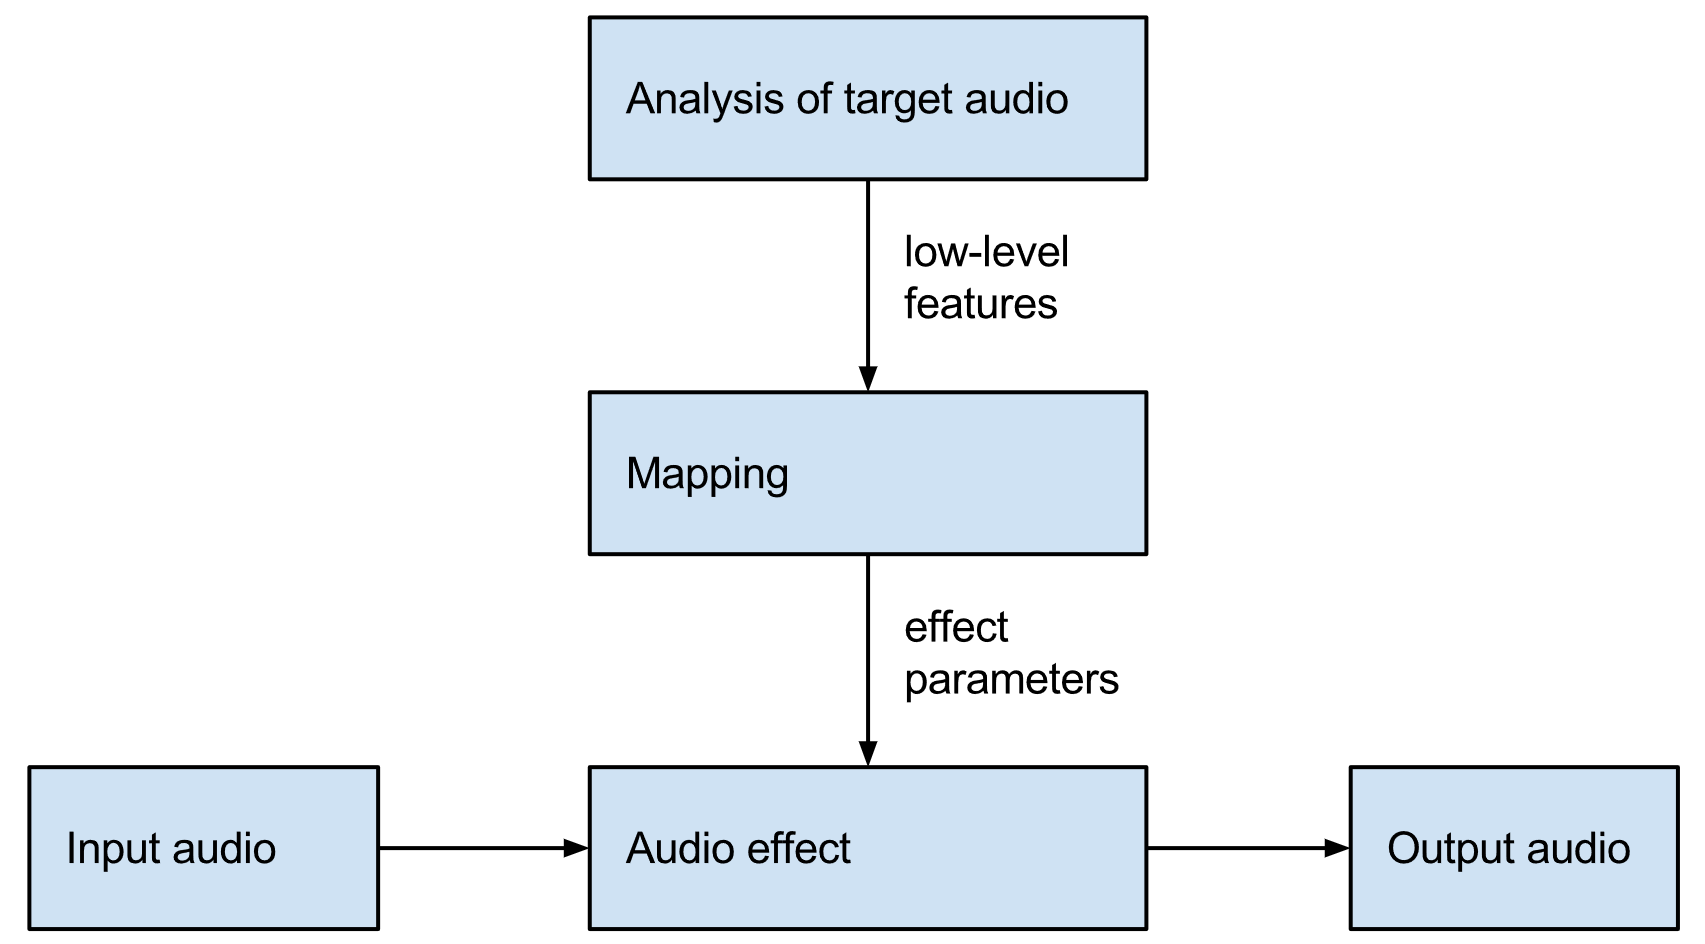
\includegraphics[width=0.6\textwidth]{01_simple_signal}
    \caption{Cross-adaptive audio effect process with two audio streams: input audio and target audio}
    \label{fig:simple_signal}
\end{figure}

In practice, a music performance that uses cross-adaptive audio effects can be a very complex, dynamic system with many signal interactions. However, to limit the scope and complexity of the problem, this project will study signal interactions between only two sounds at a time: an input sound and a target sound. A single audio effect is applied to the input sound. The parameters of this effect are dynamically informed by features from the target audio. The goal of the tool implemented in this project is to make interesting mappings from target audio analysis to audio effect parameters. Brandtsegg (2015) suggested that machine learning can be useful in this context. Generally, for a machine learning problem to be well-defined, a performance measure is needed. A good performance measure would be “how appealing does it sound?”. However, what generally sounds appealing to humans is tacit knowledge and cannot be simply described mathematically. Because there are no good objective measures of what a good cross-adaptive audio effect is, an assumption has been made in this project: If a cross-adaptive audio effect makes features of one sound audible in the other sound, then it is considered interesting. Therefore it has been decided that the objective of the system in this project should be to make the input sound similar to the target sound.

The mapping (figure 1.1) is a function that maps n-dimensional vectors (audio features) to m-dimensional vectors (effect parameters). Artificial neural networks are apt for this, as they can approximate a wide variety of continuous functions (Hornik, 1991). Backpropagation (Werbos, 1982; Lecun, Buttou, Orr, \& Müller, 1998) is an efficient algorithm for training neural networks (i.e. finding a set of useful weights for it), but it requires target values for the output nodes to compute error signals. Since no sets of target values are available for this project, and there is generally no good way of telling exactly how the mapping affects the resulting sound, it makes sense to use evolutionary computation to train the neural networks instead. That is feasible because it is possible to construct a fitness function that returns a score based on how similar two sounds are. All in all, this project is about developing a toolkit that explores evolutionary computation in various ways to evolve artificial neural networks that act as mappings in cross-adaptive audio effects.

As the developed system has many components and deals with lots of numbers in the form of audio features, neural network weights, audio effect parameters, output sounds and fitness values, it’s hard to understand what the system really does. To alleviate this, a significant part of the project has been about developing a comprehensive interactive visualization system as a part of the toolkit. One motivation for this is that one cannot improve the optimization process if one does not know where it fails. It was also made in order to make the toolkit more human-understandable and to make evaluation of results more efficient.

% !TEX encoding = UTF-8 Unicode
%!TEX root = thesis.tex
% !TEX spellcheck = en-US
%%=========================================
\chapter{Background Information}
\label{chapter:background_information}

\section{Genetic Algorithms}
Genetic algorithms \citep{goldberg1989, back1996} are iterative algorithms that can approximate solutions to optimization problems. In such problems, one usually doesn’t know how to construct a good solution, but it is possible to measure how good a solution is. The methods used in genetic algorithms are inspired by Darwin's principle of natural selection. In the algorithm, a population of individuals is simulated through generations of ``life". Each individual is a candidate solution to the optimization problem. The fittest individuals, as determined by a fitness function, are the individuals that are most likely to survive and reproduce (either asexually or sexually). Individuals that are deemed less fit are more likely to die young, and do not get to pass their genes on to future generations. During reproduction, crossover and mutation occurs. Crossover is a genetic operator that combines two parents to produce an offspring. Mutation is a genetic operator that alters an individual slightly. The whole process is roughly illustrated by figure \ref{fig:genetic_algorithm_cycle}.

\begin{figure}[H]
    \centering
    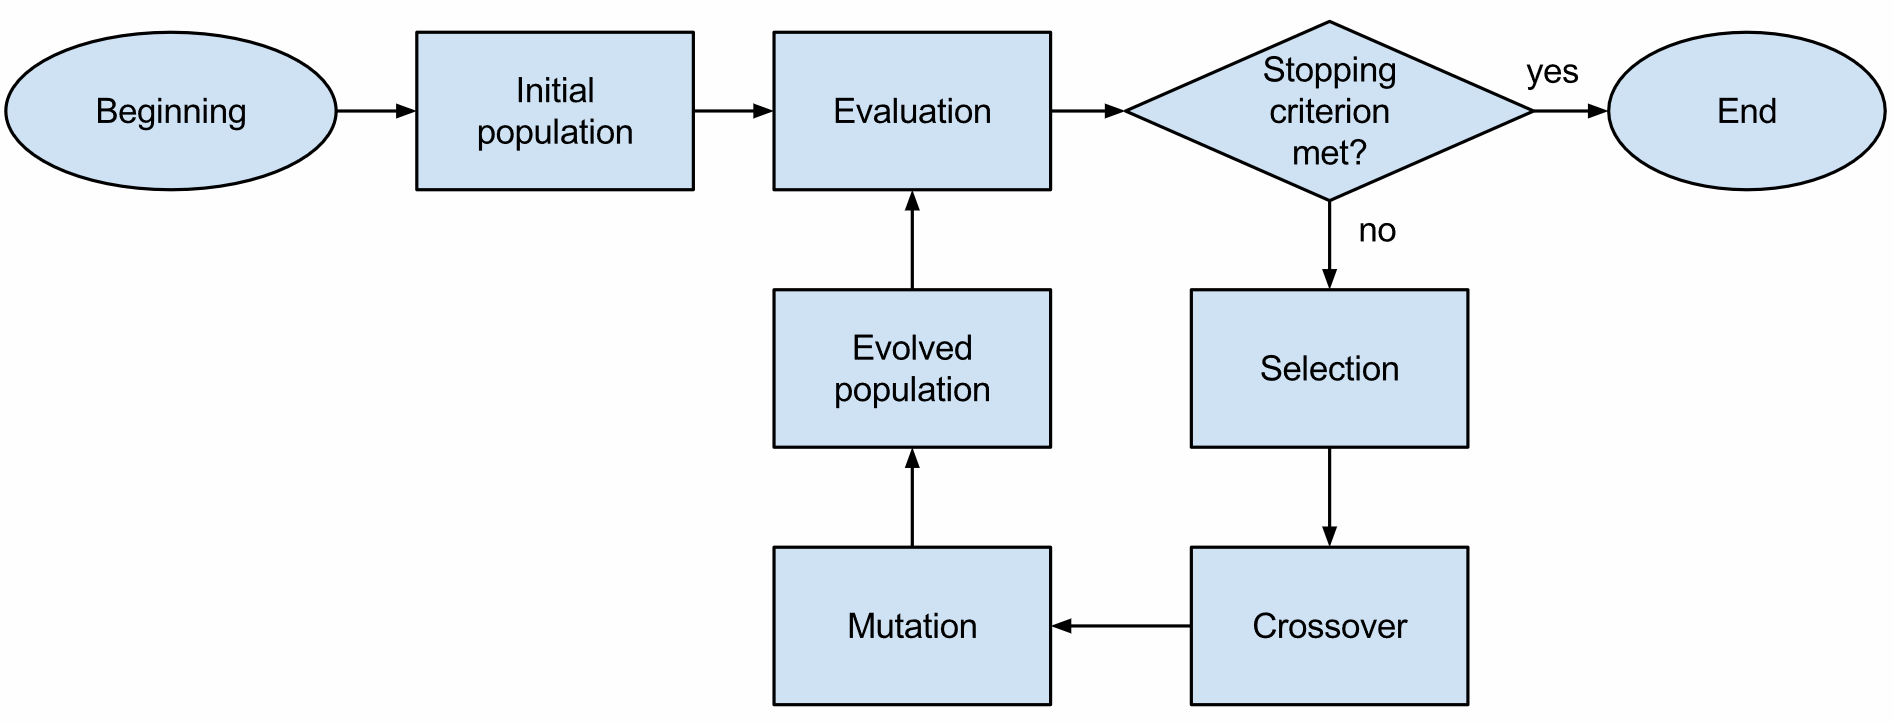
\includegraphics[width=1.0\textwidth]{02_genetic_algorithm_cycle}
    \caption{Genetic algorithm cycle}
    \label{fig:genetic_algorithm_cycle}
\end{figure}

\section{Artificial Neural Networks}
Artificial Neural Networks (ANN) are systems of interconnected ``neurons", or nodes \citep{caudill1987}. A connection from a node A to a different node B means that the activation level of node A influences the activation level of node B based on the numerical weight of the connection. The activation level of a node is calculated by adding up all incoming signals to that node and running that number through the node's activation function. An ANN can be thought of as a function that transforms n-dimensional vectors to m-dimensional vectors. Figure \ref{fig:neural_network} illustrates a simple neural network and the inner workings of one of the nodes.

\begin{figure}[H]
    \centering
    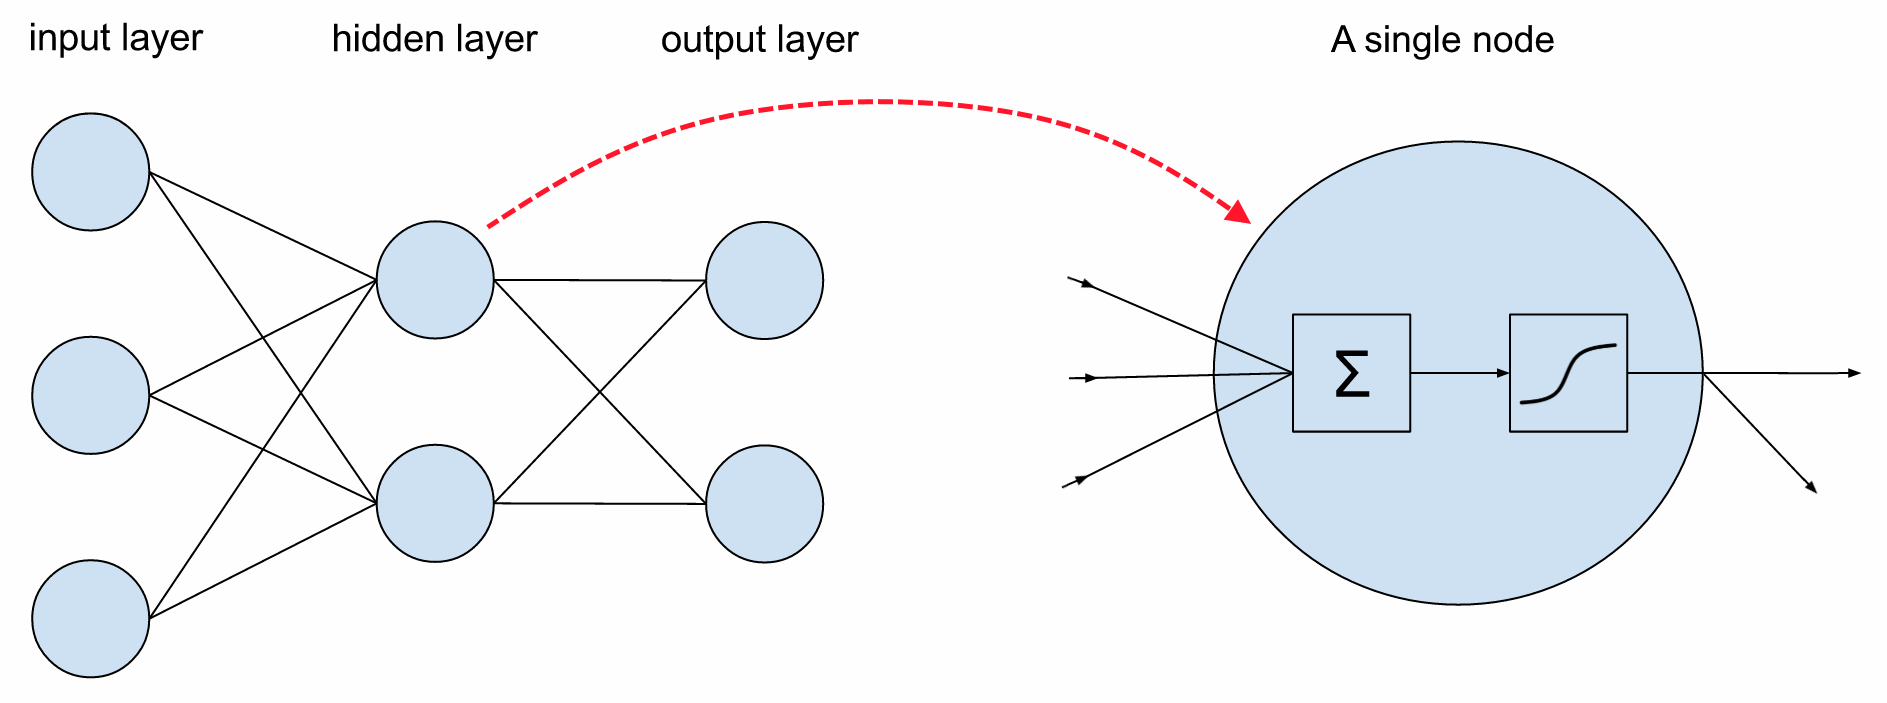
\includegraphics[width=1.0\textwidth]{neural_network}
    \caption{To the left: Illustration of a small neural network with one hidden layer. To the right: Illustration of a hidden node with sigmoid activation function}
    \label{fig:neural_network}
\end{figure}

\section{Neuroevolution}
Neuroevolution is a technique that uses evolutionary algorithms to train artificial neural networks. It differs from supervised learning algorithms such as backpropagation in that it does not require a set of correct input-output pairs. Instead, only a performance measure (fitness function) is needed.

\section{NeuroEvolution of Augmenting Topologies (NEAT)}
NEAT \citep{stanley2002} is a neuroevolution technique that evolves neural networks with genetic algorithms. Not only the weights of the ANN are evolved, but also the structure. The NEAT approach begins with a feed-forward approach with input nodes and output nodes that are fully connected. The ANN can then grow larger by having nodes and links added to it. NEAT can also remove nodes and links.

\iffalse
TODO:
Competing conventions
Species
Genotype (list of nodes, list of connections)
Phenotype
Crossover
Interspecies crossover
Dynamic compatibility
Min species
Max species
Aging species
Innovations
Young age fitness boost
Species stagnation
Competitive coevolution stagnation
Kill worst species each 15 generations
Survival rate
Elitism
Tournament selection
Sexual vs asexual reproduction?
Mutation operations
\fi

\section{Multi-Objective Evolutionary Algorithms}
As real-life problems often have more than one objective, there is a need for ways to deal with multiple objectives effectively. A multi-objective evolutionary algorithm (MOEA) is an algorithm for solving mathematical optimization problems involving more than one objective function to be optimized simultaneously \citep{veldhuizen2000}. One well-known algorithm of this kind is Nondominated Sorting Genetic Algorithm II (NSGA-II) \citep{nsga2}. In this algorithm, the performance measure is based primarily on rank and secondarily on crowding distance. Rank is calculated by running the fast non-dominated sort algorithm. This algorithms assigns a rank to each individual. If the rank of individual A is better than the rank of another individual B, it means that A dominates B. Individual A dominates B if both the following conditions are true:

\begin{itemize}  
\item The solution A is no worse than B in all objectives.
\item The solution A is strictly better than B in at least one objective.
\end{itemize}

Crowding distance is a way to measure how crowded the search space around the individual is. Crowding distance is quantified by forming a cuboid with the nearest neighbours as vertices, and then taking the average of the side lengths of the cuboid. Large crowding distances are encouraged because it preserves diversity in the population \citep{nsga2}.

\section{Audio Feature Extraction Tools}
Audio feature extraction is the process of computing a compact numerical representation that can be used to characterize a segment of audio. Low-level features such as spectral centroid and Mel-Frequency Cepstral Coefficients (MFCC) \citep{mermelstein1976, logan2000} are computed directly from the audio signal, frame by frame. A frame is a slice of audio and can consist of for example 1024 samples. In an audio signal with sampling rate 44.1 kHz, the duration of such a frame would be approximately 23 ms.

Audio features can be used in many different ways, such as music information retrieval and musical genre classification. In this project, they are used for similarity measures and for controlling the parameters of audio effects. Four audio feature extraction tools were used in this project: Aubio \citep{brossier2003aubio}, Essentia \citep{bogdanov2013essentia}, LibXtract \citep{bullock2007libxtract} and Csound \citep{csound}.

\section{Audio Effects}
Audio effects are processing techniques that alter audio so it sounds different. The following subsections describe the audio effects used in this project.

\subsection{Modified Hyperbolic Tangent}
Modified hyperbolic tangent is a waveshaping function that can model the characteristics of analog distortion, and especially tube distortion \citep{mtanh}. Modified hyperbolic tangent differs from hyperbolic tangent in that one can model the positive and the negative slopes differently. This distortion effect makes the sound ``fuzzier" by adding harmonic components. Figure \ref{fig:modified_hyperbolic_tangent_waveform_and_spectrum} illustrates an example of this.

$$\text{mtanh}(x)=\frac{e^{ax}-e^{-bx}}{e^{cx}+e^{-dx}}$$

\begin{figure}[H]
    \centering
    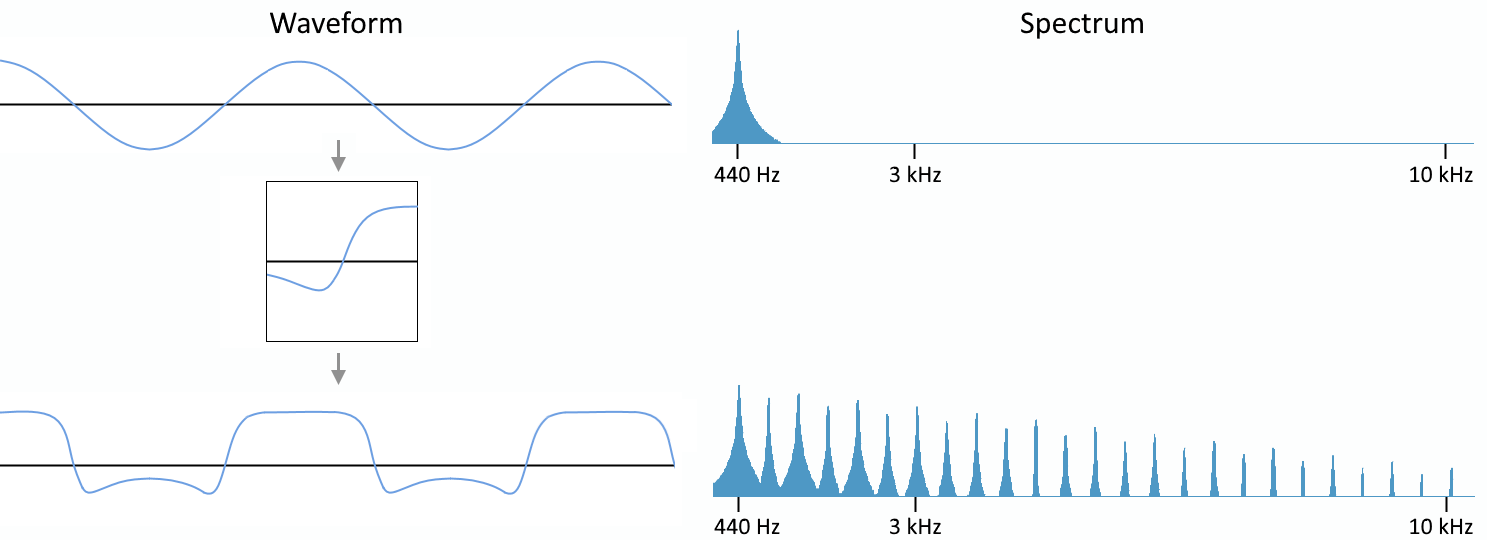
\includegraphics[width=1.0\textwidth]{modified_hyperbolic_tangent_waveform_and_spectrum}
    \caption{Harmonic frequency components are added to a 440 Hz sine wave by applying a modified hyperbolic tangent function}
    \label{fig:modified_hyperbolic_tangent_waveform_and_spectrum}
\end{figure}

\subsection{Low-Pass Filter}
A low-pass filter attenuates high frequencies and retains low frequencies unchanged \citep{dodge_jerse_1997}. It can be used to make a sound ``darker" or ``smoother" in timbre. A resonant low-pass filter is a low-pass filter that has a peak in the response curve at the cutoff frequency, as illustrated by figure \ref{fig:low_pass_filter}. This quality can be used to boost a single tone in a sound with a rich frequency spectrum. The width of the resonant peak is described by a parameter called Q. As Q increases, the resonance becomes more pronounced.

\begin{figure}[H]
    \centering
    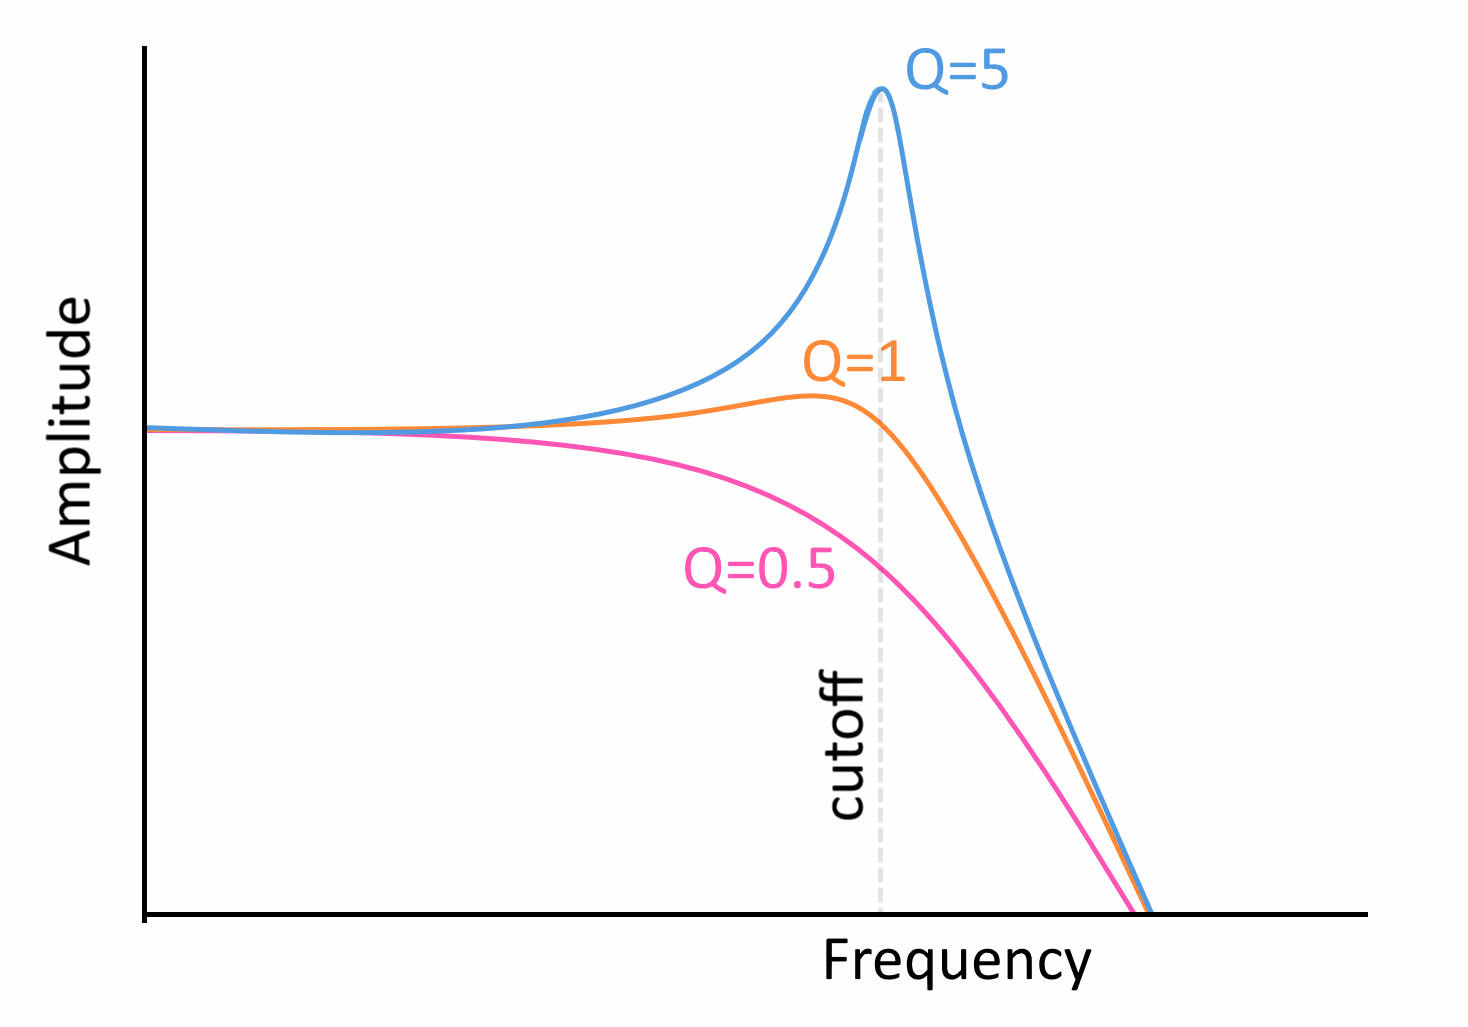
\includegraphics[width=0.5\textwidth]{05_low_pass_filter}
    \caption{Frequency response of a resonant low-pass filter with various Q values}
    \label{fig:low_pass_filter}
\end{figure}

\subsection{Band-Pass Filter}
A band-pass filter rejects frequencies outside a given range \citep{dodge_jerse_1997}. This filter has two parameters. Center frequency (denoted by $f_0$ in figure \ref{fig:bandpass}) defines the center of the frequency range. Bandwidth (denoted by $B$ in figure \ref{fig:bandpass}) defines how broad or narrow the frequency range is.

\begin{figure}[H]
    \centering
    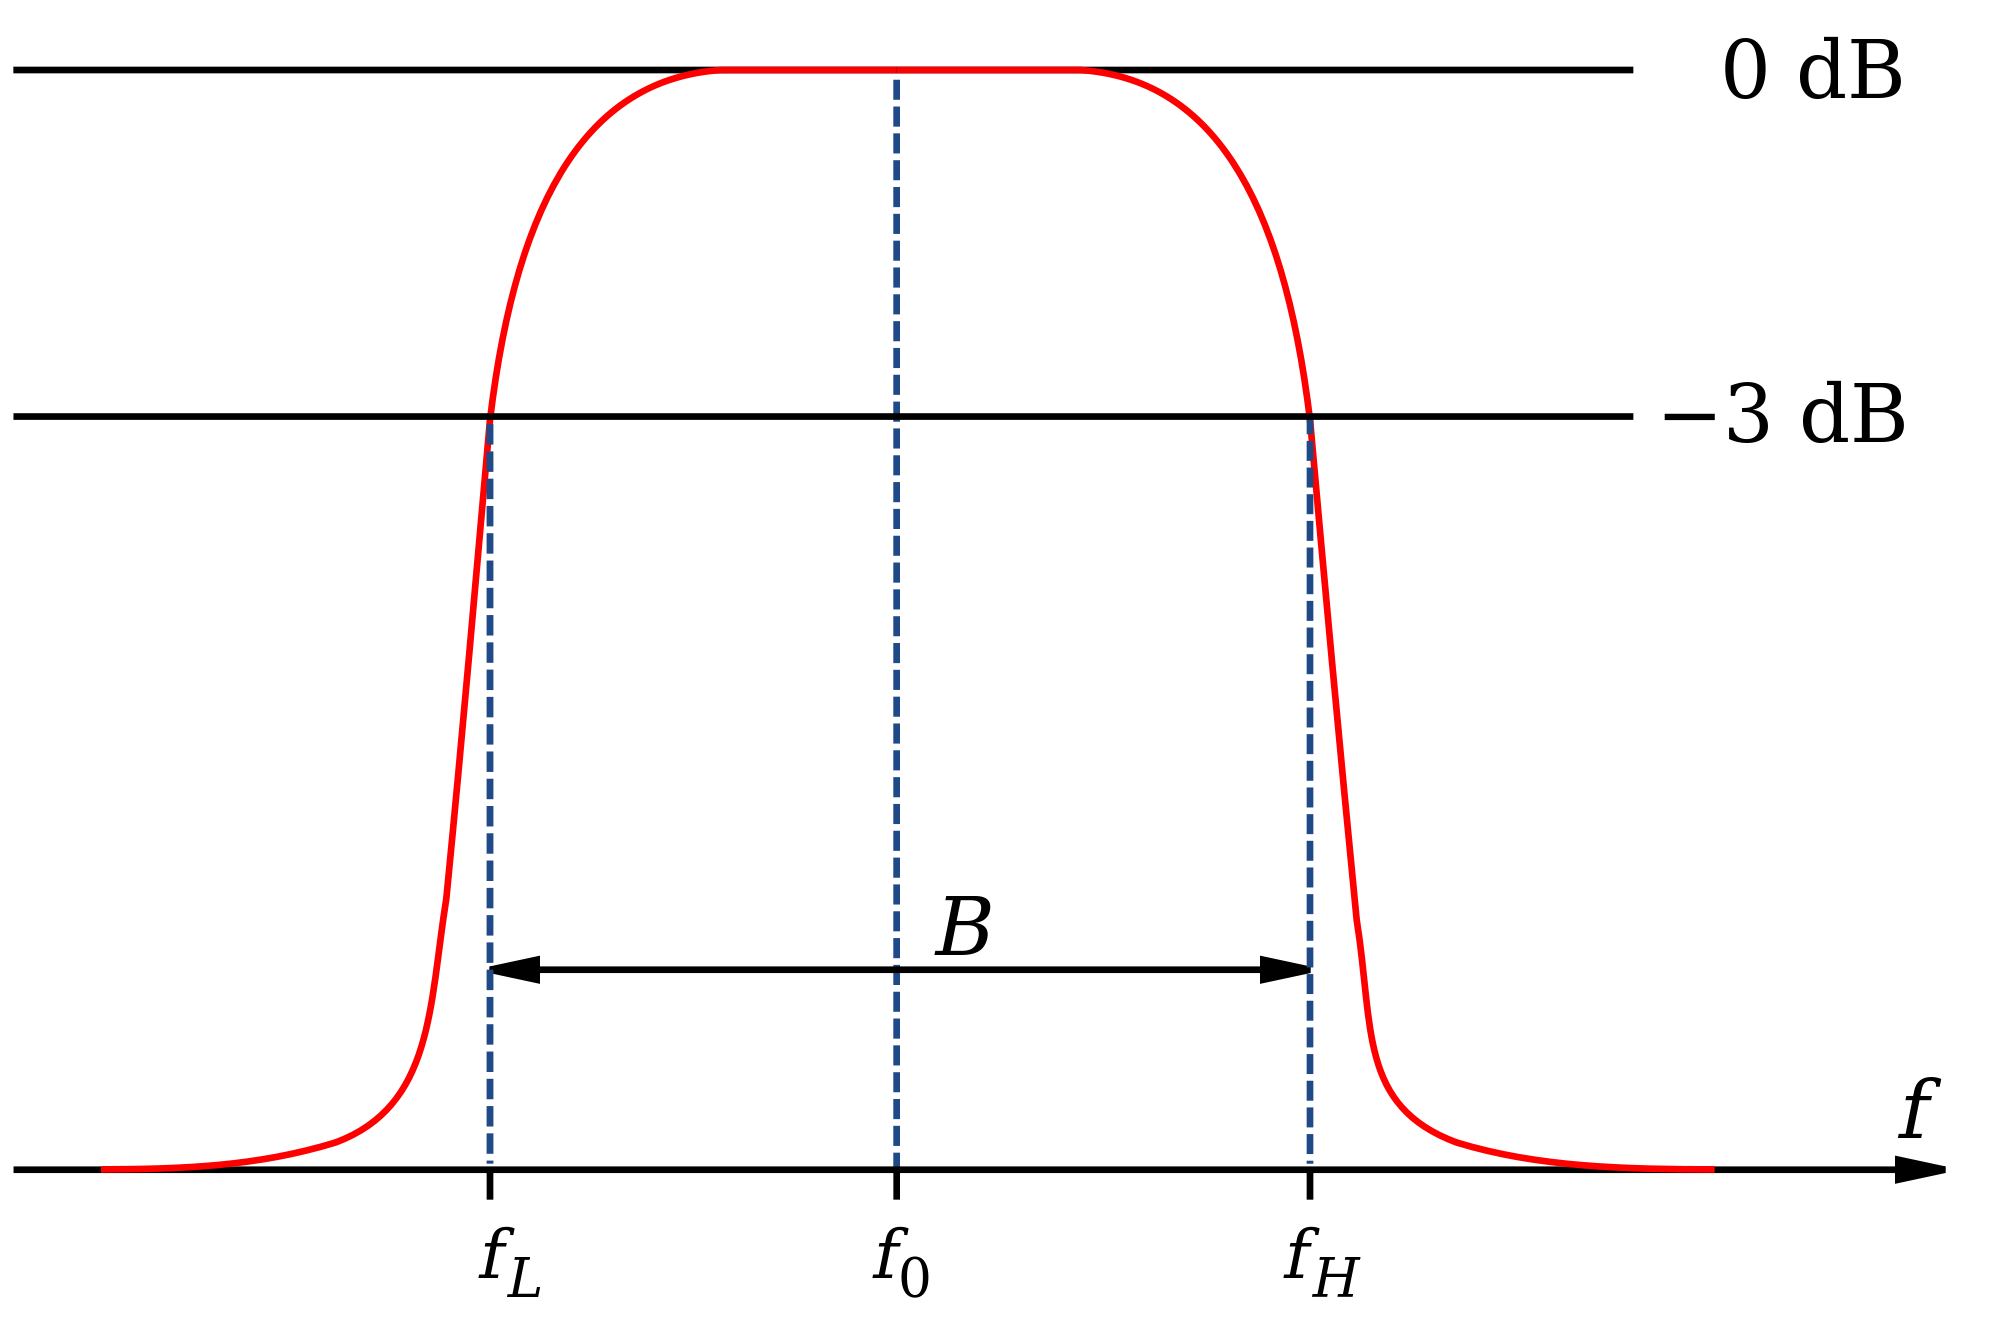
\includegraphics[width=0.5\textwidth]{bandpass}
    \caption{A diagram that illustrates the frequency response of a band-pass filter and defines its bandwidth}
    \label{fig:bandpass}
\end{figure}

\subsection{Amplitude Modulation}
The amplitude modulation effect multiplies the sound signal with a unipolar sine wave that oscillates between 0 and 1. When the frequency of the sine wave is low (\textless~20 Hz), one can hear that the amplitude is being brought up and down, as in tremolo \citep{serafin2007}. With higher frequencies there is instead an effect on the timbre of the sound. The modulator generates a set of frequency sidebands, as illustrated in figure \ref{fig:am_sidebands}

\begin{figure}[H]
    \centering
    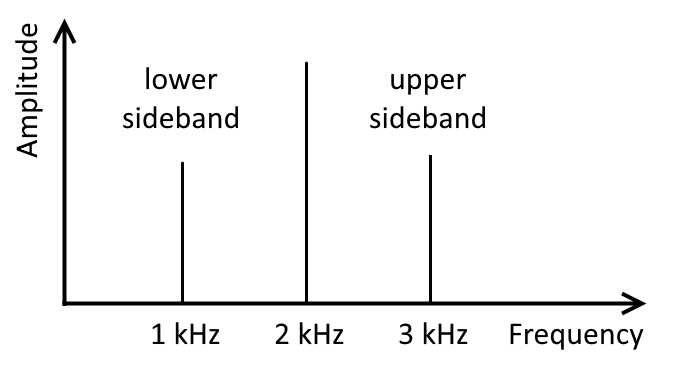
\includegraphics[width=0.5\textwidth]{am_sidebands}
    \caption{Frequency spectrum plot of a 2 kHz sine wave modulated with a 1 kHz unipolar sine wave}
    \label{fig:am_sidebands}
\end{figure}

\subsection{Bit Reduction}
The bit reduction effect reduces the number of bits used to represent a sample \citep{bitreduction}. Each sample amplitude value is rounded to a number of discrete steps. This introduces a particular kind of distortion, also called quantization noise.

\begin{figure}[H]
    \centering
    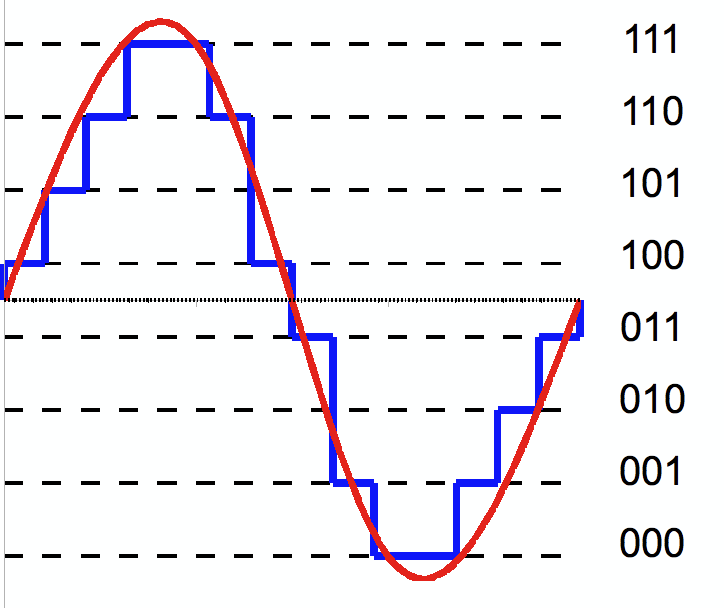
\includegraphics[width=0.3\textwidth]{bit_reduction}
    \caption{A high fidelity sine wave quantized to 3 bits per sample. \textit{By Hyacinth, CC BY-SA 3.0, \url{https://commons.wikimedia.org/w/index.php?curid=30716342}}}
    \label{fig:bit_reduction}
\end{figure}

\subsection{Chorus}
The chorus effect delays the input signal by a short \textit{delay time} (usually in the range 20-50~ms) and mixes it with the dry input signal \citep{chorus}. The \textit{delay time} is variable and usually controlled by a Low-Frequency Oscillator (LFO), as illustrated by figure \ref{fig:chorus}. This may create an impression of multiple voices playing or singing the same thing.

\begin{figure}[H]
    \centering
    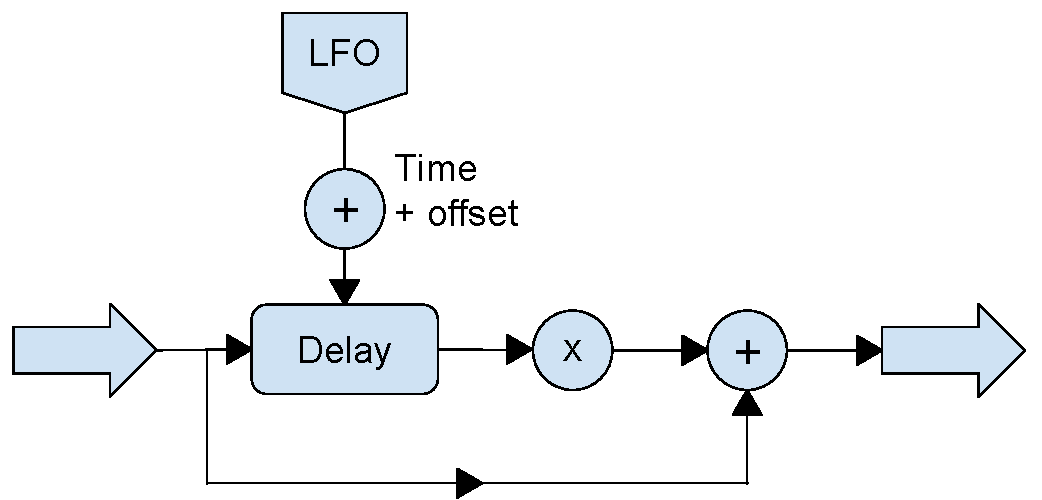
\includegraphics[width=0.5\textwidth]{chorus}
    \caption{Signal flow in a chorus effect}
    \label{fig:chorus}
\end{figure}


\section{Audio Processing Tools}
Audio processing is the alteration of audio signals, typically through audio effects. One popular audio processing tool is Csound \citep{csound}. This is both an audio programming language and a program that runs Csound code. The Csound program takes in a text file of code. This code is executed by the Csound program. The output is sound that is directed to either an audio interface (live) or to a file (non-real-time processing). Csound is used by musicians and composers, typically in experimental electroacoustic music. Traditionally, it has been an offline tool, due to lack of computational power. Today, computational power is sufficient for Csound to run in real-time, so it can be used in live settings such as concerts and sound installations. Csound can not only run on desktop computers, but can also be used as audio processing engine in mobile applications for the operating systems Android and iOS.

\section{Specialization Project}
This master's thesis is a continuation of the author's specialization project. The preliminary experiments in the specialization project were found to be successful. This led to a published paper in the proceedings of the 2nd AES Workshop on Intelligent Music Production\footnote{\url{http://www.aes-uk.org/forthcoming-meetings/wimp2/\#proceedings}}. This paper is included in appendix \ref{appendix:jordal_paper}. The author also presented his findings in a 15-minute talk at this event.

The following subsections will summarize some of the main areas of study in the experiments in the specialization project.

\subsection{Output Activation Functions}
Three different output activation functions (used in the output nodes of the neural networks) were compared. Sigmoid was found to be better than linear and sine in most cases (see figure \ref{fig:output_activation_functions_avg}).

\begin{figure}[H]
    \centering
    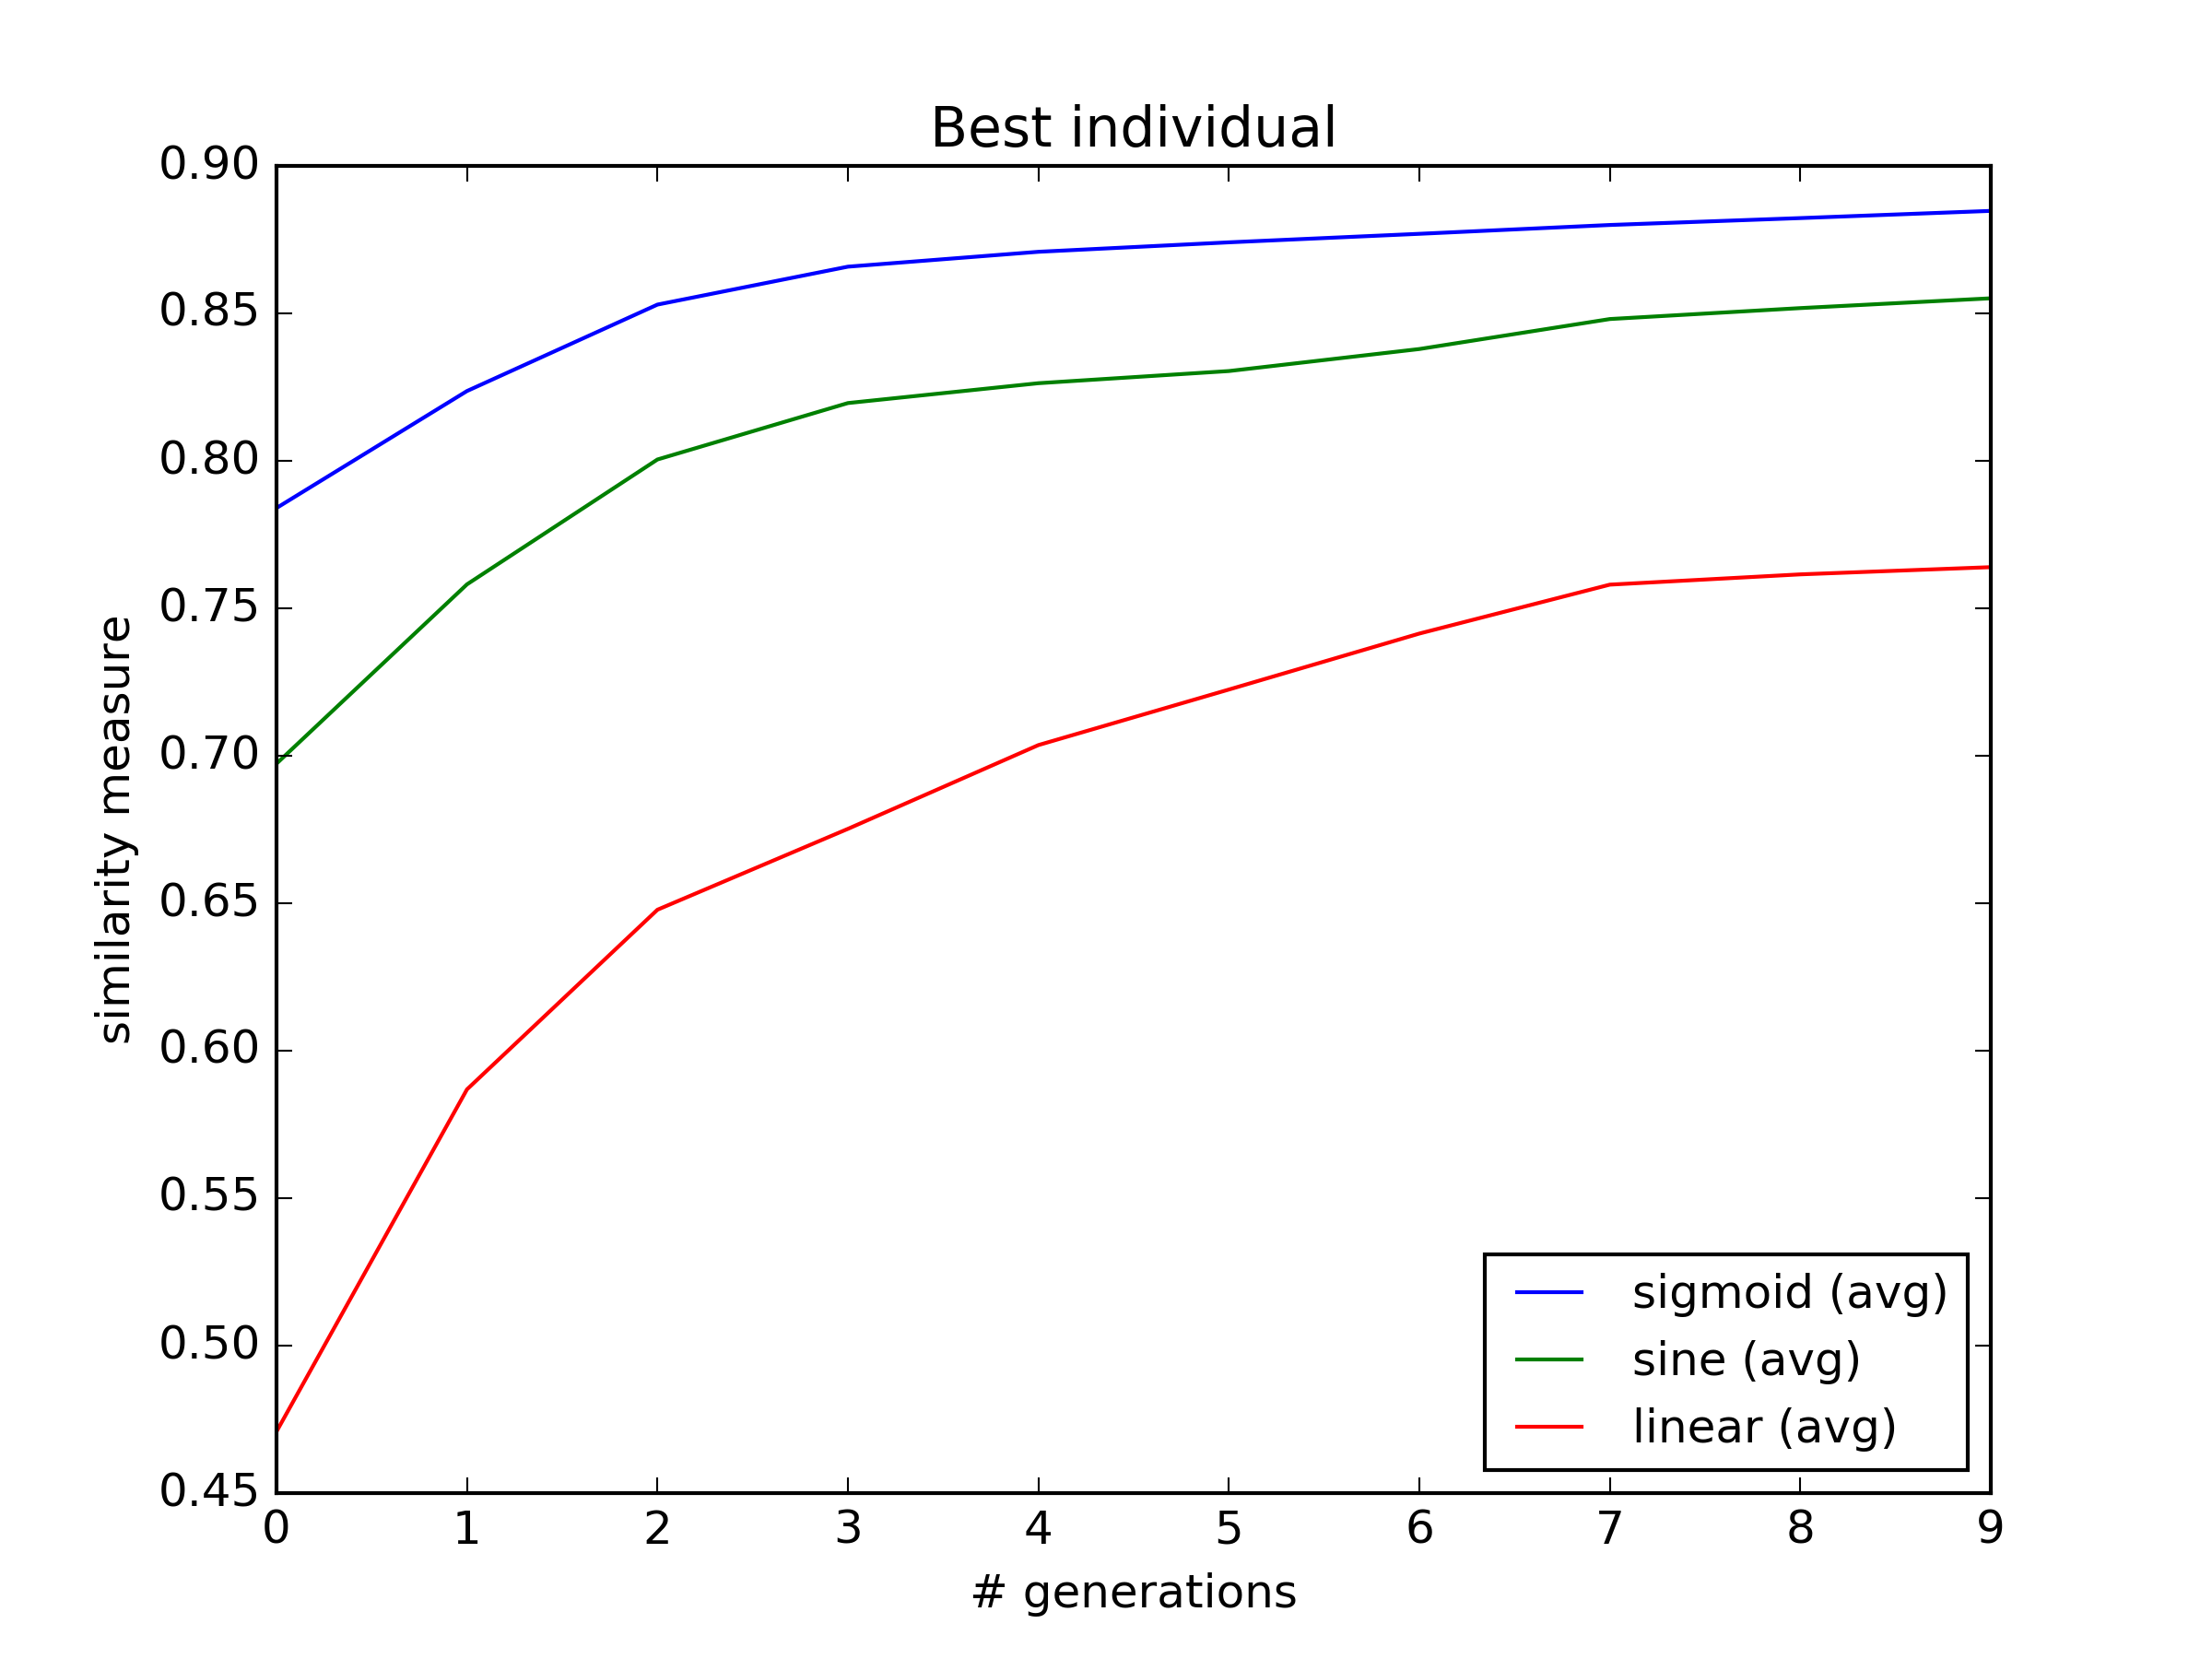
\includegraphics[width=0.85\textwidth]{output_activation_functions_avg}
    \caption{Average fitness over 20 runs}
    \label{fig:output_activation_functions_avg}
\end{figure}

\subsection{Fitness Functions}
Five fitness functions were compared. Figure \ref{fig:fitness_functions_avg} shows how well they scored on average on the similarity measure (local similarity).

\subsubsection{Local Similarity}
The local similarity fitness function is based on the average euclidean distance between the feature vector of the target sound and the output sound in the k frames of the two sounds.

\begin{verbatim}
Function LOCAL_SIMILARITY(target, individual):
    total_euclidean_distance = 0
    for each k in range(num_frames):
        A = target.get_feature_vector(k)
        C = individual.get_feature_vector(k)
        total_euclidean_distance += EUCLIDEAN_DISTANCE(A, C)
    avg_euclidean_distance = total_euclidean_distance / num_frames
    return 1 / (1 + avg_euclidean distance)
\end{verbatim}

where \texttt{EUCLIDEAN\_DISTANCE} is $d(p,q)=\sqrt{(q_1-p_1)^2+(q_2-p_2)+...+(q_n-p_n)^2}$

\subsubsection{Multi-Objective Optimization}
This fitness function is inspired by NSGA-II \citep{nsga2}. It incorporates two measures: rank and crowding distance. These are concepts taken directly from the NSGA-II paper, and they are then used in a math expression that satisfies these two constraints that are used in NSGA-II:

\begin{itemize}
\item $\text{rank}(A) > \text{rank}(B) \implies \text{fitness}(A) > \text{fitness}(B)$
\item $\text{rank}(A) = \text{rank}(B), \text{CD}(A) > \text{CD}(B) \implies \text{fitness}(A) > \text{fitness}(B)$
\\ where CD stands for crowding distance
\end{itemize}

The ranks of the individual are calculated by doing non-dominated sort. Crowding distance is computed between individuals in a given rank. The multi objective fitness function works like this:

\begin{Verbatim}[fontsize=\small]
Function MULTI_OBJECTIVE(target, individuals):
    for individual in individuals:
        CALCULATE_OBJECTIVES(individual, target)
    fronts = FAST_NON_DOMINATED_SORT(individuals)
    for rank in fronts:
        CALCULATE_CROWDING_DISTANCE(fronts[rank])  # assigns individual.crowding_distance
        for individual in fronts[rank]:
            individual.fitness = 1.0 / (rank + (0.5 / (1.0 + individual.crowding_distance)))

Function CALCULATE_OBJECTIVES(individual, target):
    individual.objectives = {}
    for feature in similarity_features:
        individual.objectives[feature] = EUCLIDEAN_DISTANCE(
                                             target.analysis[feature],
                                             output.analysis[feature])
\end{Verbatim}

Pseudocode for \texttt{FAST\_NON\_DOMINATED\_SORT} and \texttt{CALCULATE\_CROWDING\_DISTANCE} can be found in the NSGA-II paper \citep{nsga2}.

\subsubsection{Hybrid}
While NSGA-II is good at optimizing for non-dominated individuals, these individuals may be extreme tradeoffs and therefore not necessarily feasible solutions in practice. In order to reward good tradeoffs more, the author developed the hybrid fitness function. This fitness function returns the average of \texttt{MULTI\_OBJECTIVE} and \texttt{LOCAL\_SIMILARITY}.

\subsubsection{Novelty Search}
Novelty search \citep{lehman2008} ignores the objective and optimizes for novelty instead. The reason that this may work well is that in some problems the intermediate steps to the goal do not resemble the goal itself. When it comes to implementation, MultiNEAT has novelty search built-in, but Python bindings for it are missing, so the author could not use it in his Python application. However, novelty search can be implemented on top of most evolutionary algorithms, by using a fitness function that rewards novelty \citep{noveltysearchwebsite}, so that is what the author did. First, each individual needs to be represented as a vector that describes its characteristics. This vector is constructed by concatenating all audio feature series of the individual. The implemented fitness function assigns high fitness values to the individuals that have long euclidean distances from the 3 nearest neighbours, where the neighbours are individuals that have been evaluated earlier. The very first population gets random fitness values, because there are no earlier individuals to measure distance from.

\subsubsection{Mixed}
This fitness function is simple: For each generation, one of the following fitness functions is chosen randomly and applied: local similarity, multi-objective, hybrid, novelty. The idea behind this fitness function is to create a dynamic fitness landscape, where the individuals that get good scores from all fitness functions have the greatest chance of survival over time.

\begin{figure}[H]
    \centering
    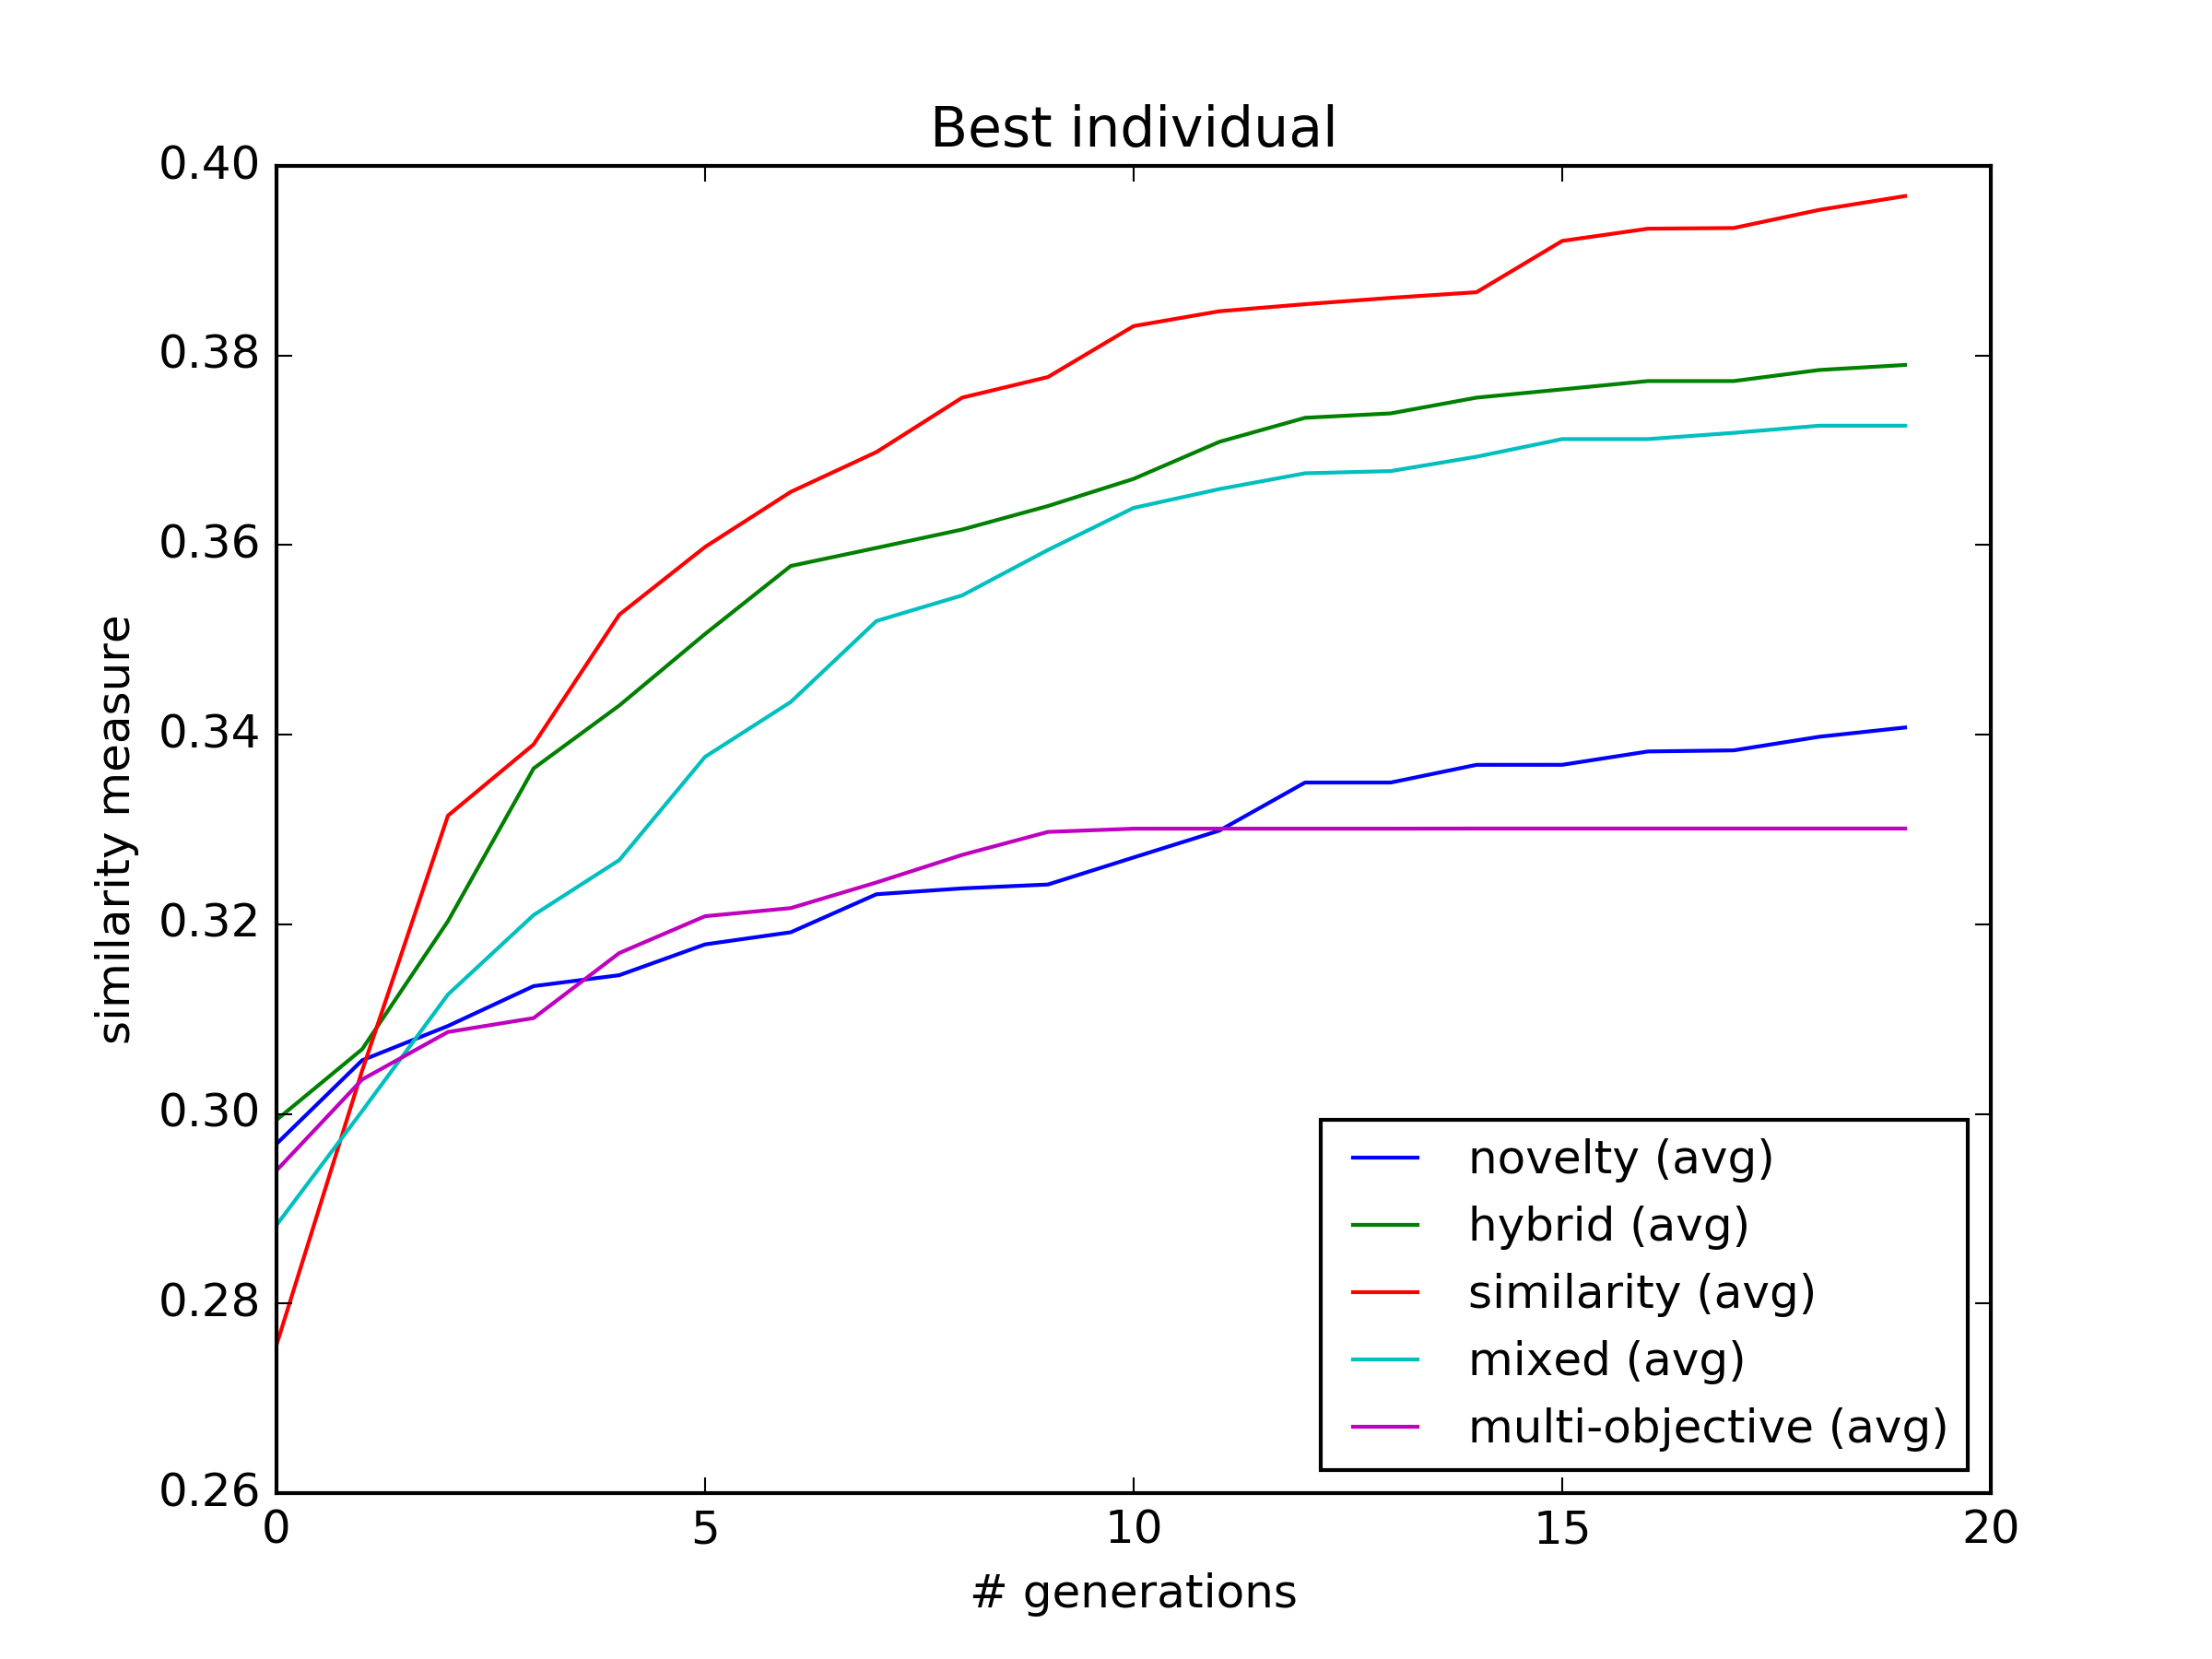
\includegraphics[width=0.85\textwidth]{fitness_functions_avg}
    \caption{Best individual on average over 20 runs, with 20 generations for each run}
    \label{fig:fitness_functions_avg}
\end{figure}

\subsection{Automatic Feature Selection}
When dealing with high-dimensional input data, the number of weights in a fully connected neural network becomes quite large. Clean and useful combinations of all the input signals can be hard to evolve. To deal with this situation, one can use Feature Selective NeuroEvolution of Augmenting Topologies (FS-NEAT) \citep{whiteson2005}. This NEAT variation starts with just a few connections and gradually adds/removes connections.

In an experiment with noise for input sound and a sine sweep for output sound, FS-NEAT was found to perform better than classic NEAT. This experiment had 68 audio features as input. Classic NEAT would typically evolve a very noisy parameter control, so the output sounds became glitchy and not very musically interesting. FS-NEAT has been found to deal with the high-dimensional input more effectively, as it selected only a few of the audio features that were useful for getting high fitness values. Figure \ref{fig:neat_vs_fs_neat_avg_max} shows fitness values with NEAT and FS-NEAT in the described experiment.

\begin{figure}[H]
    \centering
    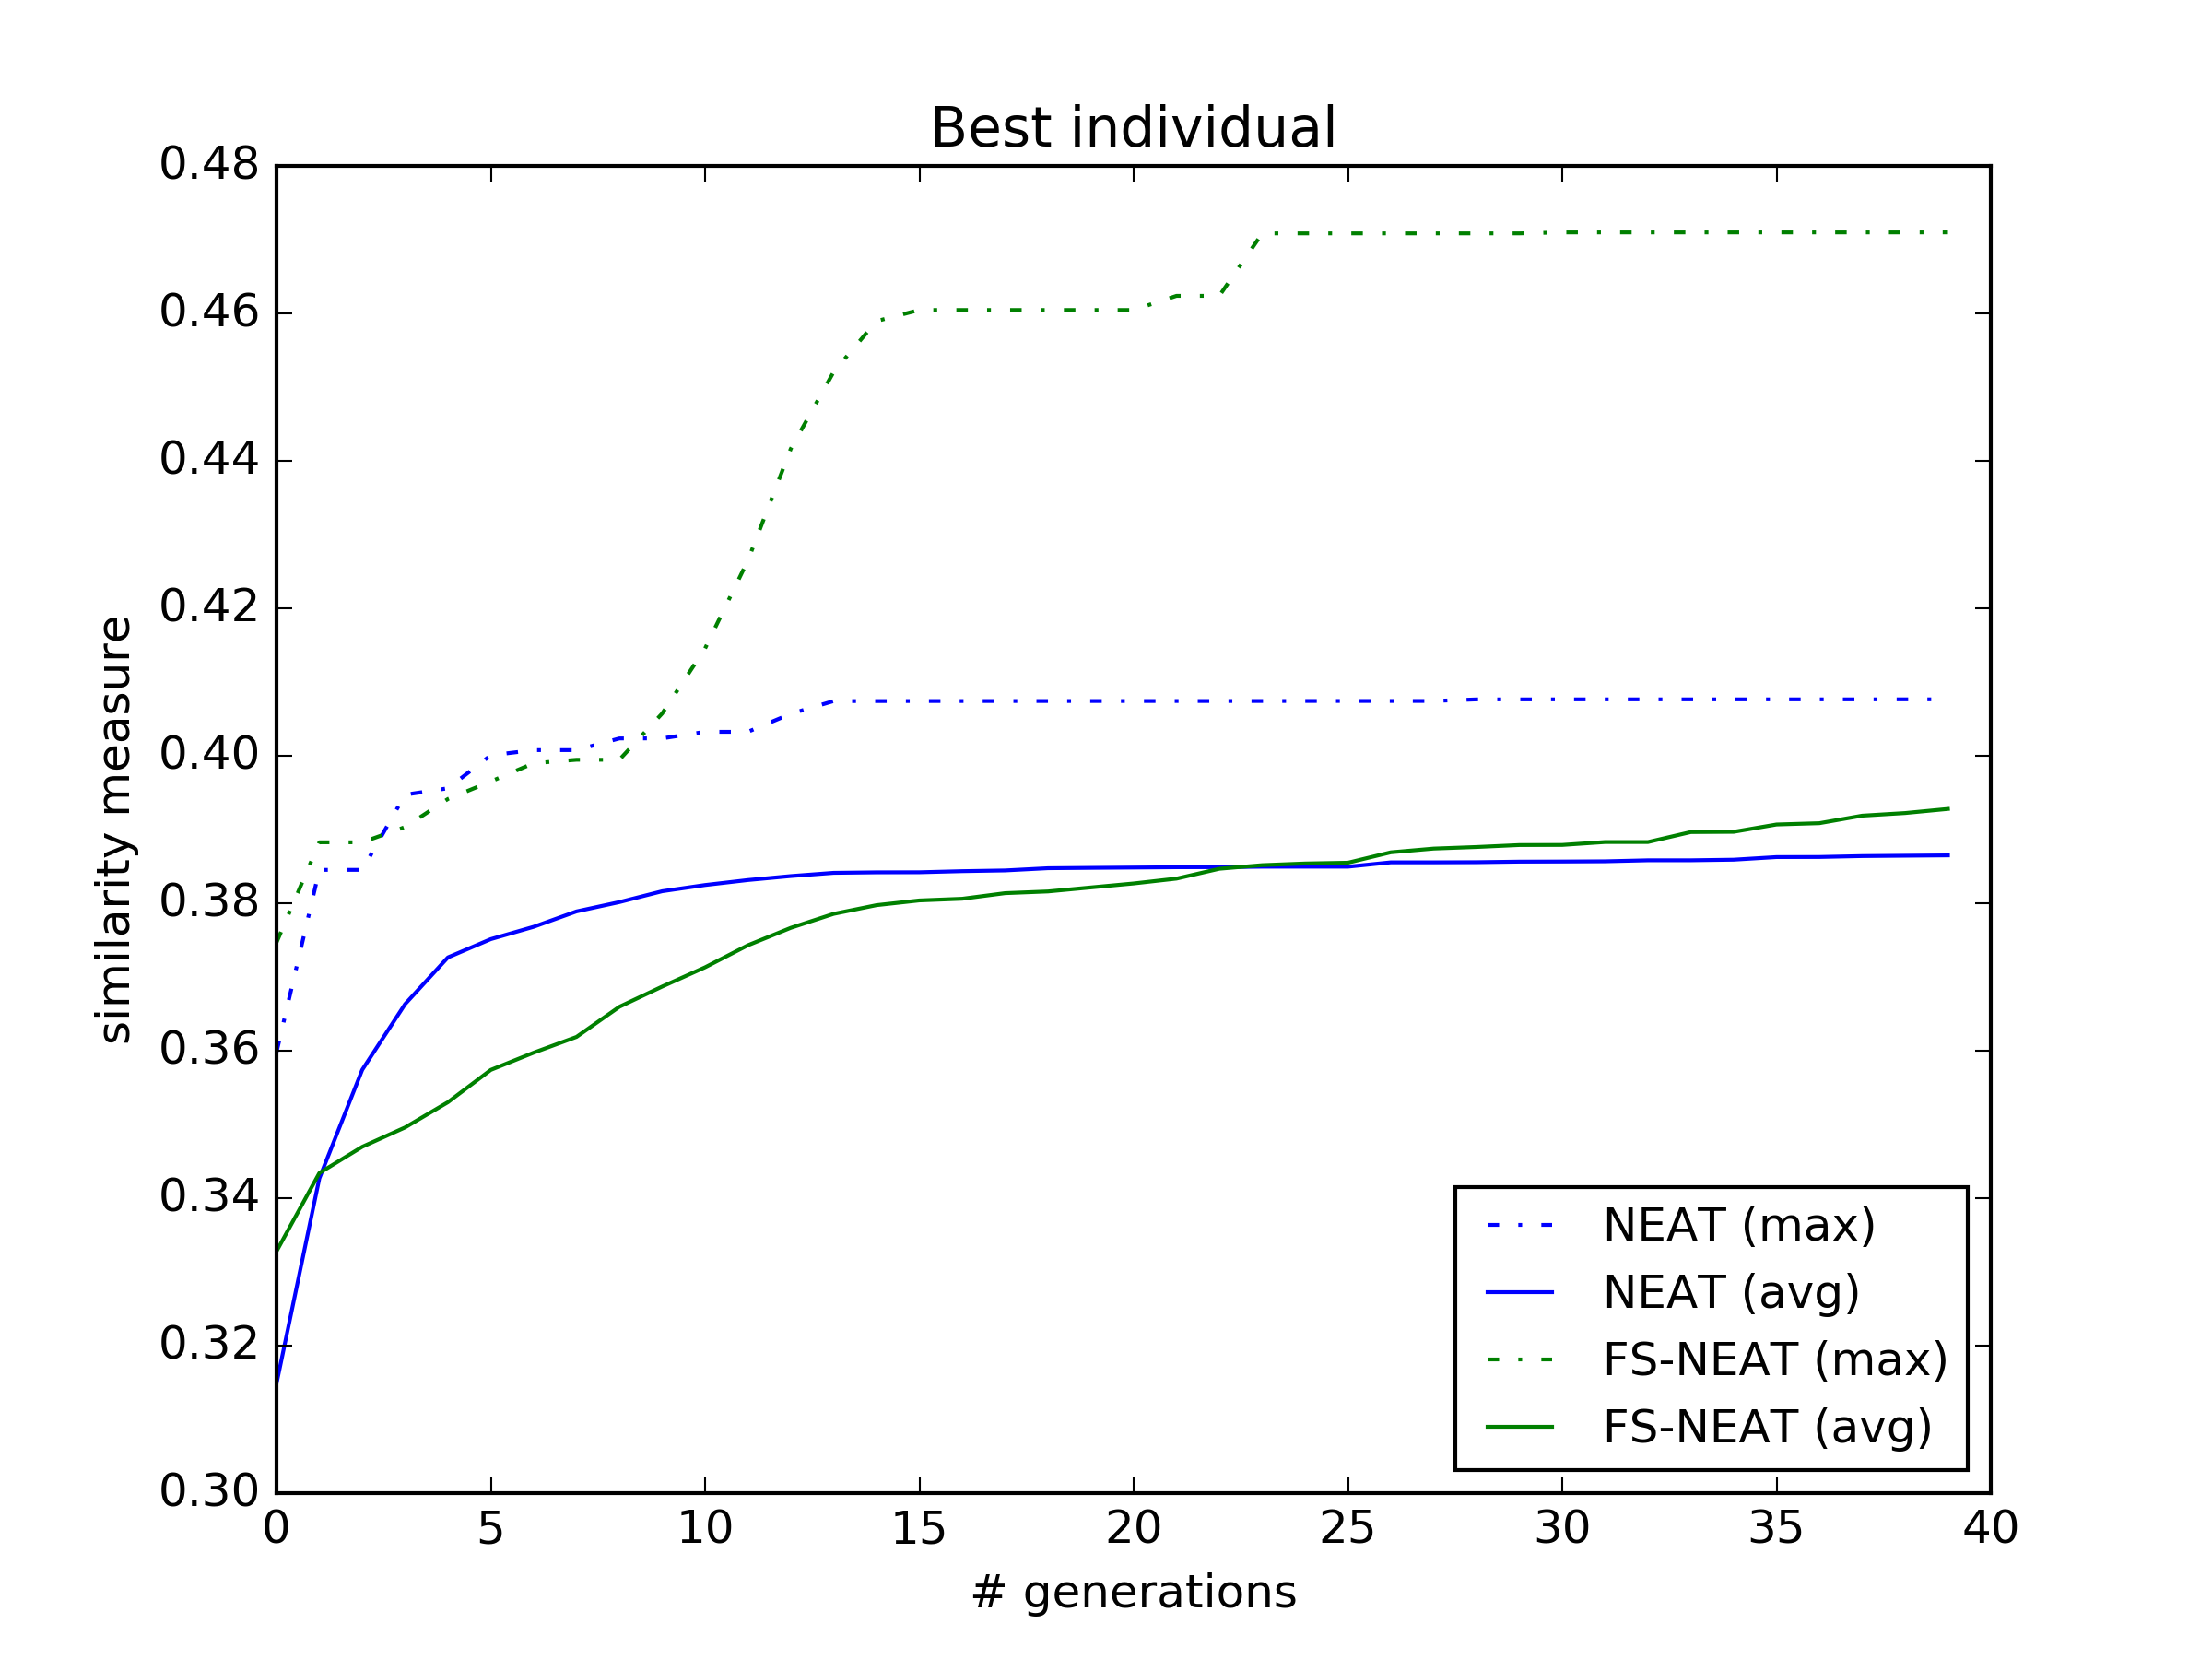
\includegraphics[width=0.85\textwidth]{neat_vs_fs_neat_avg_max}
    \caption{Fitness values in runs with NEAT and FS-NEAT, aggregated from 20 runs with each configuration.}
    \label{fig:neat_vs_fs_neat_avg_max}
\end{figure}




% !TEX encoding = UTF-8 Unicode
%!TEX root = thesis.tex
% !TEX spellcheck = en-US
%%=========================================
\addcontentsline{toc}{section}{Acknowledgment}
\section*{Acknowledgment}
I would like to thank the following persons for their great help during \ldots

If the project has been carried out in cooperation with an external partner (e.g., a company), you should acknowledge the contribution and give thanks to the involved persons.

You should also acknowledge the contributions made by your supervisor(s).

\begin{flushright}
O.N.\\[1pc]
(Your initials)
\end{flushright}
\tableofcontents
\setcounter{page}{0}
\pagenumbering{arabic}
% !TEX encoding = UTF-8 Unicode
%!TEX root = thesis.tex
% !TEX spellcheck = en-US
%%=========================================
\chapter{Introduction}
The first chapter of a well-structured thesis is always an introduction, setting the scene with background, problem description, objectives, limitations, and then looking ahead to summarize what is in the rest of the report. This is the part that readers look at first---\emph{so make sure it hooks them!}

%%=========================================
\section{Background}
In this section, you should present the problem that you are going to investigate or analyze; why this problem is of interest; what has, so far, been done to solve the problem, and which parts of the problem that remain.

{\color{red}Below, I have set up some headings (subsection titles) without a number. These are included to help you remember to cover the related issues. The headings should be removed in your final print.}
%%=========================================
\subsection*{Problem Formulation}
You should define your problem in a clear an unambiguous way and explain why this is a problem, why it is of interest---and to whom. It is also important to delimit the problem area.
%%=========================================
\subsection*{Literature Survey}
You should here present the main books and articles that treat problems that are similar to what  you are studying. If you,  later in your thesis, describe the ``state of the art'' -- with a detailed literature survey, you may just give a very brief survey here (approx. a quarter of a page). If this is the only literature survey, you need to go into more details. An objective of the literature survey is to show the reader that you are familiar with the main literature within your field of research -- so that you do not ``reinvent the wheel.''


References to literature can be given in two different ways:
\begin{itemize}
\item As an \emph{explicit} reference: It is shown by \citet{lundteigen08} and partly also by \citet{rausand14}  that \ldots.
\item As an \emph{implicit} reference: It is shown \citep[e.g., see][Chap. 4]{rausand04} that \ldots.
\end{itemize}
In the example above, we have used ``author-year'' references, which is the preferred format. 
\begin{remark}
Following agreement with your supervisor, you may also refer by numbers, for example,  [1]. To do this, open the file \texttt{ramsstyle.sty} and  comment out (by \%) the command \texttt{$\backslash$usepackage\{natbib\}} and un-comment the corresponding command \texttt{$\backslash$usepackage[numbers]\{natbib\}}.\footnote{Notice the strange way we have to write the ``backslash'' in the text. This is because the ``backslash'' is a command in \LaTeX.}
\end{remark}
 You may include a link to the Internet in the text or in a footnote by using a command like: \url{http://www.ntnu.edu/ross}. 

When you refer to the scientific literature, you should always write in \emph{present} tense. Example: \citet{rausand04} show that \ldots.

\begin{remark}
Hyperlinks are included by the command \texttt{$\backslash$usepackage\{hyperref}\} in \texttt{ramsstyle.sty}. If you feel that the hyperlinks are disturbing when you enter the text, or want to avoid the hyperlinks in printed text, you may either comment out or edit this command in \texttt{ramsstyle.sty}.
\end{remark}
%%=========================================
\subsection*{What Remains to be Done?}
After you have defined and delimited your problem -- and presented the relevant results found in the literature within this field, you should sum up which parts of the problem that remain to be solved.
%%=========================================
\section{Objectives}
The main objectives of this Master's project are
\begin{enumerate}
\item This is the first objective
\item This is the second objective
\item This is the third objective
\item More objectives
\end{enumerate}

The objectives shall be written as \emph{fundamental objectives} telling what to do and not \emph{means objectives} telling how to do it.

All objectives shall be stated such that we, after having read the thesis, can see whether or not you have met the objective. ``To become familiar with \ldots'' is therefore not a suitable objective.

%%=========================================
\section{Limitations}
In this section you describe the limitations of your study. These may be related to the study object (physical limitations, operational limitations), to the environmental and operational conditions, to the thoroughness of the analysis, and so on.
%%=========================================
\section{Approach}
Here you should describe the (scientific) approach that you will use to solve the problem and meet your objectives. You should specify the approach for each objective.

If there are any ethical problems related to your approach, these should be highlighted and discussed.
%%=========================================
\section{Structure of the Report}
The rest of the report is organized as follows. Chapter 2 gives an introduction to \ldots

\begin{remark}
Notice that chapter and section headings shall be written in lowercase, but that all main words should start with a capital letter.
\end{remark}


The report should be no longer than \underline{60 pages} in this format (+ the CV).
% !TEX encoding = UTF-8 Unicode
%!TEX root = thesis.tex
% !TEX spellcheck = en-US
%%=========================================
\chapter[Equations, etc]{Equations, Figures, and Tables}
The content of Chapter 2 will vary with the topic of your thesis. This chapter only gives guidance to some technical aspects of \LaTeX.
 
\begin{remark}
If you want a shorter chapter or section title to appear in the Table of Contents and in the headings of the chapter, you just include the short title in square brackets before the title of the chapter/section. Example: \begin{verbatim}\section[Short Title]{Long Title}\end{verbatim}.
\end{remark}

%%=========================================
\section{Simple Equations}
Mathematical symbols and equations can written in the text as $\lambda$, $F(t)$, or even $F(t)=\int_0^t \exp(-\lambda x)\,dx$, or as displayed equations
\begin{equation}
F(t)=\int_0^t \exp(-\lambda x)\,dx
\label{eq1}
\end{equation}


The displayed equations are automatically given equation numbers -- here (\ref{eq1}) since this is the first equation in Chapter 2. Note that you can refer to the equation by referring to the ``label'' you specified as part of the equation environment.

You can also include equations without numbers:
\begin{equation*}
F(t)=\sum_{i=1}^n \binom{n}{i}\sin(i\cdot t)
\end{equation*}

%%=========================================
\subsection*{More Advanced Formulas}
Long formulas that cannot fit into a single line can be written by using the environment \texttt{align} as
\begin{align}
F(t)&= \sum_{i=1}^n \sin(t^{n-1}) - \sum_{i=1}^n \binom{n}{i}\sin(i\cdot t) \\
      & + \int_0^\infty n^{-x} e^{-\lambda x^t}\,dt
\end{align}

In some cases, you need to write ordinary letters inside the equations. You should then use the commands 
\begin{verbatim}
\textrm  and/or \mathrm
\end{verbatim}
The first command returns the normal text font and will be scaled automatically, while the second command will be scaled according to the use.
\begin{equation*}
\textrm{MTTF}= \int_0^\infty R_\mathrm{avg}(t)\,dt
\end{equation*}



Please consult the \LaTeX\ documentation for further details about mathematics in \LaTeX.
%%=========================================
\section*{Definitions}
If you want to include a definition of a term/concept in the text, I have made the following macro (see in \texttt{ramsstyle.sty}):
\begin{defin}
\textbf{Reliability}: The ability of an item to perform a required function under stated environmental and operational conditions and for a stated period of time.\newline
\end{defin}
When text is following directly after the definition, it may sometimes be necessary to end the definition text by the command
\begin{verbatim}
\newline
\end{verbatim}
I have not included this in the definition of the \texttt{defin} environment to avoid too much space when there is not a text-block following the definition.
%%=========================================
\section{Including Figures}
If you use pdf\LaTeX\ (as recommended), all the figures must be in pdf, png, or jpg format. We recommend you to use the pdf format.  Please place the figure files in the directory \textbf{fig}. Figures are included by the command shown for Figure~\ref{fig1}. Please notice the ``path'' to the figure file written by a \emph{forward} slash (/). You should not include the format of the figure file (pdg, png, or jpg) -- just write the ``name'' of the figure. 
\begin{figure}
\centering

\includegraphics[scale=0.6,angle=15]{fig/NTNU}
\caption{This is the logo of NTNU (rotated 15 degrees).}
\label{fig1}
\end{figure}

Each figure should include a unique \emph{label} as shown in the command for Figure~\ref{fig1}. You can then refer to the figure by the \emph{ref} command.
Notice that you can scale the size of the figure by the option \texttt{scale=k}. You may also define a specific width or height of the figure by replacing the \texttt{scale} options by \texttt{width=k} or \texttt{height=k}. The factor \texttt{k} can here be specified in mm, cm, pc, and many other length measures. You may also give \texttt{k} as a fraction of the width of the text or of the height of the text, for example, \texttt{width=0.45$\backslash$textwidth}. If you later change the margins of the text, the figure width will change accordingly. As illustrated in Figure~\ref{fig1}, you may also rotate the figure -- and also do many other things (please check the documentation of the package \texttt{graphicx} -- it is available on your computer, or you may find it on the Internet).

In \LaTeX\ all figures are floating objects and will normally be placed at the top of a page. This is the standard option in all scientific reports. If you insist on placing the figure exactly where you declare the figure, you may include the command \texttt{[h]} (here) immediately after $\backslash$\texttt{begin\{figure\}}. If you will force the figure to be located either at the top or bottom of the page, you may alternatively use  \texttt{[t]} or \texttt{[b]}. For more options, check the documentation.

Large figures may be included as a \emph{sidewaysfigure} as shown in Figure~\ref{fig2}:\footnote{You can use a similar command for large tables.}
\begin{sidewaysfigure}
\centering

\includegraphics[scale=1.8]{fig/NTNU}
\caption{This is the logo of NTNU.}
\label{fig2}
\end{sidewaysfigure}

%%=========================================
\section{Including Tables}
\LaTeX\ has a lot of different options to include tables. Only one of them is illustrated here.

\begin{table}
	\centering\small
	\caption{The degree of newness of technology.}
	\label{tab1}
		\begin{tabular*}{\textwidth}{@{\extracolsep{\fill}}lccc}
			\toprule
			  &\multicolumn{3}{c}{Level of technology maturity}\\
  \cmidrule{2-4}
			Experience with the		   &  & Limited field history or not & New or \\
              operating  condition  & Proven &  used by company/user & unproven \\
        
			\midrule
			  Previous experience & 1 & 2 & 3 \\
		          No experience by company/user & 2 & 3 & 4 \\
		          No industry experience & 3 & 4 & 4 \\
			\bottomrule
		\end{tabular*}
\end{table}

\begin{remark}
Notice that figure captions (Figure text) shall be located \emph{below} the figure -- and that the caption of tables shall be \emph{above} the table. This is done by placing the $\backslash$\texttt{caption} command beneath the command $\backslash$\texttt{includegraphics} for figures, and above the command $\backslash$\texttt{begin\{tabular*\}} for tables.
\end{remark}
%%=========================================
\section{Copying Figures and Tables}
In some cases, it may be relevant to include figures and tables from from other publications in your report. This can be a direct copy or that you retype the table or redraw the figure. In both cases, you should include a reference to the source in the figure or table caption. The caption might then be written as: \textsl{Figure/Table xx: The caption text is coming here \citep{rausand04}.}

In other cases, you get the idea from a figure or table in a publication, but modify the figure/table to fit your purpose. If the change is significant, your caption should have the following format: \textsl{Figure/Table xx: The caption text is coming here \citep[adapted from][]{rausand04}.}

%%=========================================
\section{References to Figures and Tables}
Remember that all figures and tables shall be referred to and explained/discussed in the text. If a figure/table is not referred to in the text, it shall be deleted from the report.
%%=========================================
\section{A Word About Font-encoding}
When you press a button (or a combination of buttons) on your keyboard, this is represented in your computer according to the \emph{font-encoding} that has been set up. A wide range of font-encodings are available and it may be difficult to choose the ``best'' one. In the template, I have set up a font-encoding called UTF-8 which is a modern and very comprehensive encoding and is expected to be the standard encoding in the future. Before you start using this template, you should open the Preferences ->Editor dialogue in TeXworks (or TeXShop if you use a Mac) and check that encoding UTF-8 has been specified. 

If you use only numbers and letters used in standard English text, it is not very important which encoding you are using, but if you write the Norwegian letters æ, ø, å and accented letters, such as é and ä, you may run into problems if you use different encodings. Please be careful if you cut and paste text from other word-processors or editors into your \LaTeX\ file!

\subsubsection*{Warning}
If you (accidentally) open your file in another editor and this editor is set up with another font-encoding, your non-standard letters will likely come out wrong. If you do this, and detect the error, be sure \emph{not} to save your file in this editor!!

This is not a specific \LaTeX\ problem. You will run into the same problem with all editors and word-processors -- and it is of special importance if you use computers with different platforms (Windows, OSX, Linux).

%%=========================================
\section{Plagiarism}
Plagiarism is defined as ``use, without giving reasonable and appropriate credit to or acknowledging the author or source, of another person's original work, whether such work is made up of code, formulas, ideas, language, research, strategies, writing or other form'', and is a very serious issue in all academic work. You should adhere to the following rules:
\begin{itemize}
\item Give proper references to all the sources you are using as a basis for your work. The references should be give to the original work and not to newer sources that mention the original sources.
\item You may copy paragraphs up to 50 words when you include a proper reference. In doing so, you should place the copied text in inverted commas (i.e., ``Copied text follows \ldots''). Another option is to write the copied text as a quotation, for example:
\begin{quote}
Birnbaum's measure of reliability importance of component $i$ at time $t$ is equal to the probability that the system is in such a state at time $t$ that component $i$ is critical for the system.\newline \mbox{} \hfill \citet{rausand04}
\end{quote}
\end{itemize}




% !TEX encoding = UTF-8 Unicode
%!TEX root = thesis.tex
% !TEX spellcheck = en-US
%%=========================================
\chapter[Summary]{Summary and Recommendations for Further Work}
%%This is the last chapter
In this final chapter you should sum up what you have done and which results you have got. You should also discuss your findings, and give recommendations for further work.

%%=========================================
\section{Summary and Conclusions}
Here, you present a brief summary of your work and list the main results you have got. You should give comments to each of the objectives in Chapter 1 and state whether or not you have met the objective. If you have not met the objective, you should explain why (e.g., data not available, too difficult).

This section is similar to the Summary and Conclusions in the beginning of your report, but more detailed---referring to the the various sections in the report.

%%=========================================
\section{Discussion}
Here, you may discuss your findings, their strengths and limitations.
%%=========================================
\section{Recommendations for Further Work}
You should give recommendations to possible extensions to your work. The recommendations should be as specific as possible, preferably with an objective and an indication of a possible approach.

The recommendations may be classified as:
\begin{itemize}
\item Short-term
\item Medium-term
\item Long-term
\end{itemize}
% Include more chapters as required.
%%=========================================
\appendix
% !TEX encoding = UTF-8 Unicode
%!TEX root = thesis.tex
% !TEX spellcheck = en-US
%%=========================================

\chapter{Acronyms}
\begin{description}
\item[FTA] Fault tree analysis
\item[MTTF] Mean time to failure
\item[RAMS] Reliability, availability, maintainability, and safety
\end{description}
% !TEX encoding = UTF-8 Unicode
%!TEX root = thesis.tex
% !TEX spellcheck = en-US
%%=========================================

\chapter{Additional Information}
This is an example of an Appendix. You can write an Appendix in the same way as a chapter, with sections, subsections, and so on.

%%=========================================
\section{Introduction}

%%=========================================
\subsection{More Details}
% Include more appendices as required.
%%=========================================
\bibliographystyle{apa}
\addcontentsline{toc}{chapter}{\bibname}
\bibliography{refs}  
%%=========================================

\end{document}
